\documentclass[11pt,a4paper]{article}

\usepackage[utf8]{inputenc}
\usepackage[T1]{fontenc}
\usepackage[margin=2.4cm]{geometry}
\usepackage{amsmath,amssymb}
\usepackage{graphicx}
\usepackage{booktabs}
\usepackage{caption}
\usepackage{subcaption}
\usepackage{xcolor}
\usepackage{hyperref}
\usepackage[protrusion=true,expansion=false]{microtype}
\usepackage{enumitem}
\usepackage{titlesec}

\hypersetup{colorlinks=true,linkcolor=black!70!blue,urlcolor=blue!60!black}

\titleformat{\section}{\large\bfseries}{\thesection.}{0.6em}{}
\titleformat{\subsection}{\normalsize\bfseries}{\thesubsection}{0.5em}{}
\titlespacing*{\section}{0pt}{1.0em}{0.4em}
\titlespacing*{\subsection}{0pt}{0.7em}{0.2em}

\setlength{\parindent}{0pt}
\setlength{\parskip}{0.4em}
\captionsetup{font=small,labelfont=bf,skip=4pt}

\title{\vspace{-1.5em}\textbf{Time-Varying Covariates in Mortgage Survival:\\
The Andersen--Gill Cox Extension}\\[0.3em]
\large IR\&C Assignment 3, Part E(ii) --- Spring 2026}
\author{Yueqi Lin\\\small MTH 9877, Baruch College}
\date{May 2026}

\begin{document}
\maketitle
\vspace{-1.2em}

% =================================================================
\section{Introduction}
% =================================================================

Standard Cox proportional hazards models fix all covariates at loan origination.
This is inadequate for mortgage prepayment, where the key driver --- the rate incentive
$r_{\text{orig}} - r_{\text{market}}(t)$ --- changes every month as market rates fluctuate.
A borrower who locked in at 3\% in 2020 had a strong refinancing incentive at origination;
by 2023, as market rates rose to 7\%, that same loan's incentive collapsed to $-4$\,pp,
making refinancing strictly dominated. A static model cannot represent this transition.

The \textbf{Andersen--Gill} (1982) extension resolves this by replacing one row per loan
with one row per loan-month, updating covariates at each interval.

% =================================================================
\section{Data and Feature Engineering}
% =================================================================

\textbf{Sample}: 100,000 loans drawn from the monthly panel (stratified by vintage year),
yielding 4,676,598 loan-month intervals (average $\approx$47 months per loan).

\textbf{Features} (13 total): nine static origination features (FICO, LTV, DTI, UPB,
\texttt{orig\_rate}, loan purpose dummies, occupancy dummies) shared by both models,
plus four time-varying features updated monthly in TV Cox:
\texttt{rate\_incentive}, \texttt{unemployment}, \texttt{hpi\_yoy},
and the synthetic current LTV (\texttt{ELTV}).
The static Cox baseline uses the nine shared static features plus origination-era
\texttt{unemployment} and \texttt{hpi\_yoy} (11 features total).
\texttt{mortgage\_rate} is excluded from both models: since
\texttt{rate\_incentive} $= r_{\text{orig}} - r_{\text{market}}(t)$ and $r_{\text{orig}}$
is fixed per loan, including both would create perfect within-loan collinearity.

\textbf{Synthetic ELTV} is computed monthly as:
\begin{equation}
    \text{ELTV}_t = \text{LTV}_0
    \times \underbrace{\frac{(1+r)^{360}-(1+r)^t}{(1+r)^{360}-1}}_{\text{remaining balance fraction}}
    \div \underbrace{\prod_{s=1}^{t}\!\left(1 + \frac{\text{hpi\_yoy}_s}{1200}\right)}_{\text{cumulative HPI}},
\end{equation}
capturing equity build from scheduled amortisation and home-price appreciation ---
the two dominant drivers of the refinancing put option.

\begin{figure}[h]
    \centering
    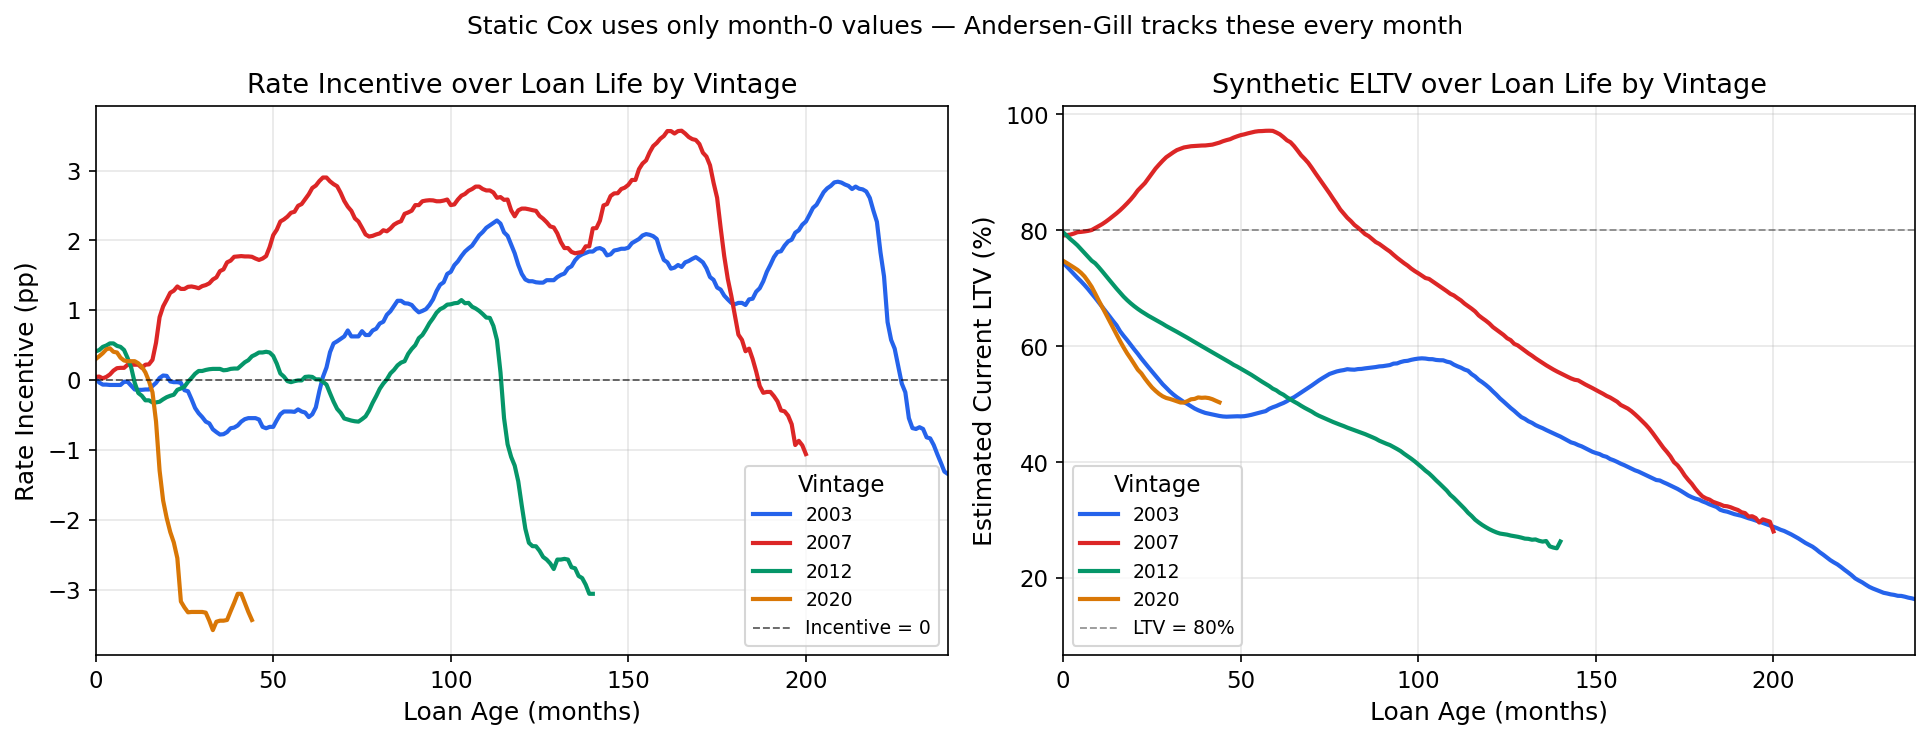
\includegraphics[width=\linewidth]{processed/Eii_tv_feature_trajectories}
    \caption{Median rate incentive (left) and ELTV (right) by vintage cohort over loan age.
      A static Cox model uses only month-0 values; the Andersen--Gill model tracks the full path.
      The 2020-vintage rate incentive turns negative within 3 years as market rates surged to 7\%,
      while 2007-vintage ELTV rises steeply as home prices recover.}
\end{figure}

% =================================================================
\section{The Andersen--Gill Model}
% =================================================================

\subsection{Hazard function}

Each loan contributes one counting-process interval $(t_{\text{start}},\, t_{\text{stop}}]$
per calendar month with the current covariate vector $\mathbf{x}_i(t)$:
\begin{equation}
    h_i(t) = h_0(t)\,\exp\!\bigl(\boldsymbol{\beta}^\top \mathbf{x}_i(t)\bigr).
\end{equation}

\subsection{Partial likelihood}

\begin{equation}
    \ell(\boldsymbol{\beta}) = \sum_{i:\,\delta_i=1}
    \Biggl[\boldsymbol{\beta}^\top \mathbf{x}_i(t_i)
    - \log \!\sum_{j \in \mathcal{R}(t_i)}
    \exp\!\bigl(\boldsymbol{\beta}^\top \mathbf{x}_j(t_i)\bigr)\Biggr],
\end{equation}
where $\mathcal{R}(t_i)$ is the set of all loan-months still active just before $t_i$.
The key difference from the standard Cox partial likelihood is that each loan may contribute
\emph{multiple} intervals to the risk set, and $\mathbf{x}_i(t)$ is updated at each.

\subsection{Landmark C-index}

For time-varying models, the overall C-index conflates event timing with event probability.
We instead compute the \textbf{landmark C-index} at fixed horizons $t^*$:
\begin{equation}
    C(t^*) = P\!\left(\hat{h}_i(t^*) > \hat{h}_j(t^*) \;\Big|\; T_i \leq t^* < T_j\right),
\end{equation}
where each loan's score $\hat{h}_i(t^*) = \exp\!\bigl(\hat{\boldsymbol{\beta}}^\top \mathbf{x}_i(\min(T_i, t^*))\bigr)$
uses its covariate state at the landmark time. This aligns with Part B's per-horizon AUC evaluation.

% =================================================================
\section{Results}
% =================================================================

\subsection{Coefficient comparison}

\begin{figure}[h]
    \centering
    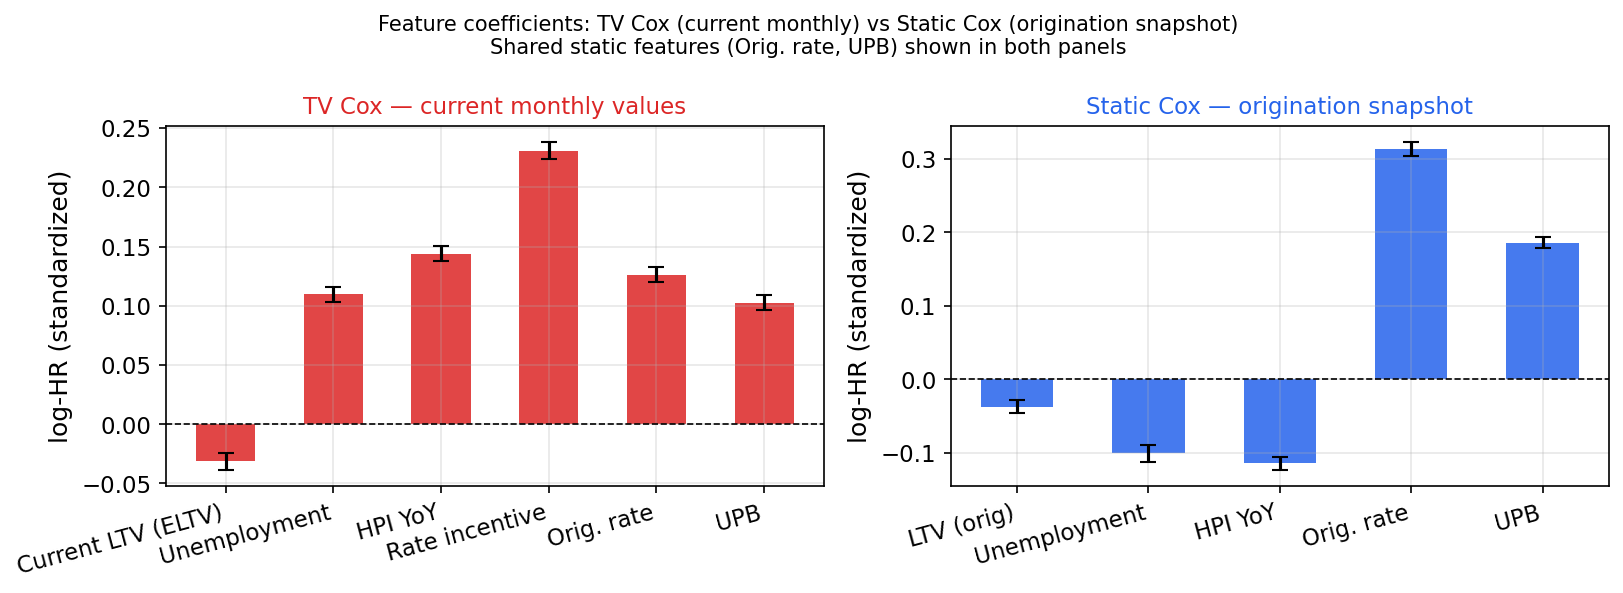
\includegraphics[width=0.88\linewidth]{processed/Eii_static_vs_tv}
    \caption{Coefficient comparison: TV Cox (left, red --- 4 time-varying + \texttt{orig\_rate} + UPB)
      vs.\ static Cox (right, blue --- 2 origination-era macro + \texttt{orig\_rate} + UPB).
      \texttt{orig\_rate} and UPB are shared static features shown in both panels.
      Both macro signals flip sign from static to TV Cox --- high-unemployment origination
      cohorts pre-date Fed easing, while current high-unemployment months coincide with low rates.}
\end{figure}

\begin{figure}[h]
    \centering
    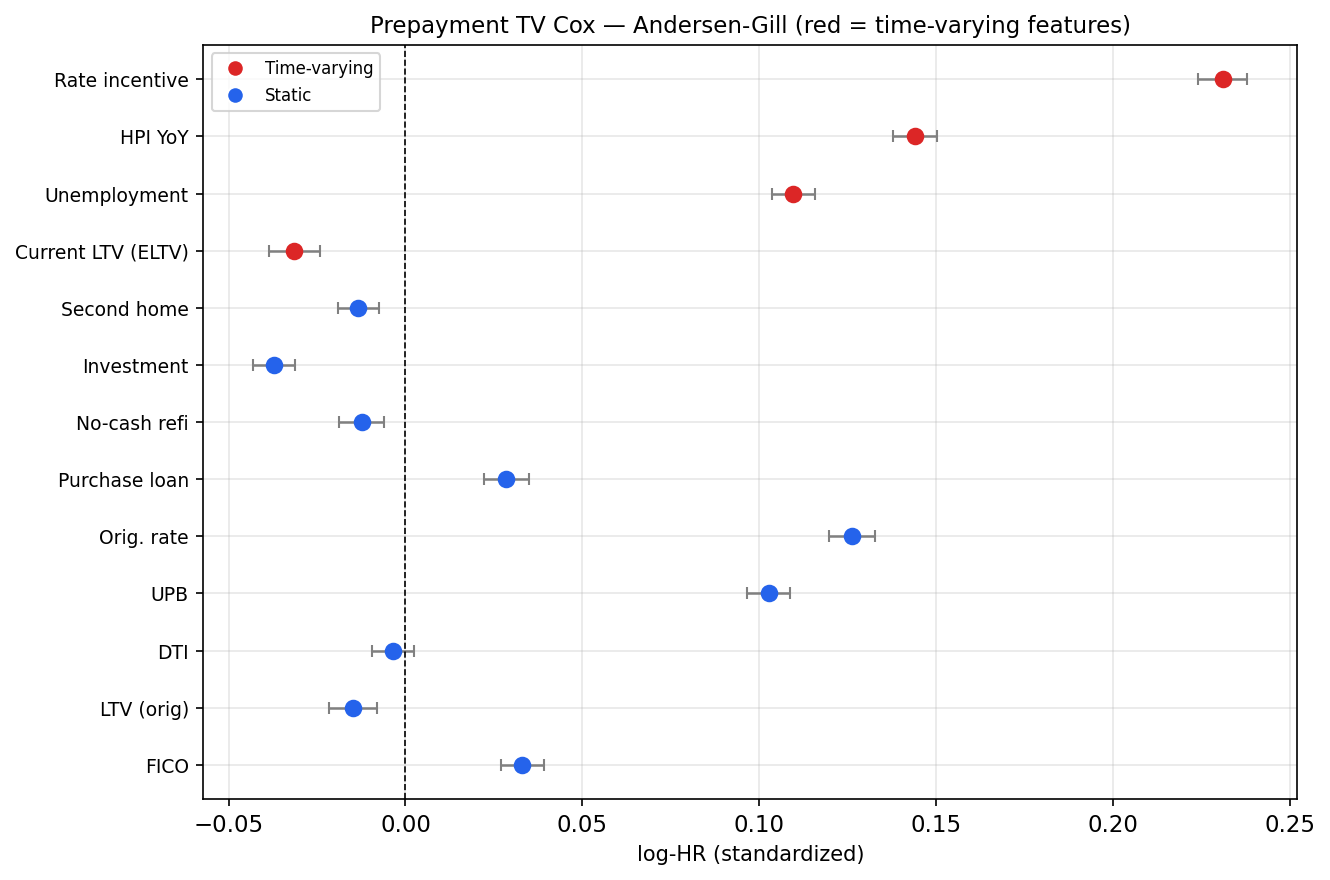
\includegraphics[width=\linewidth]{processed/Eii_tv_cox_forest}
    \caption{TV Cox forest plot. Red markers: time-varying features;
      blue markers: static origination features.
      \texttt{rate\_incentive} is the dominant positive predictor of prepayment;
      \texttt{ELTV} is negative (high current LTV suppresses refinancing).}
\end{figure}

\begin{center}
\small
\begin{tabular}{lccp{5.4cm}}
\toprule
\textbf{Feature} & \textbf{Static Cox} & \textbf{TV Cox} & \textbf{Economic reading} \\
\midrule
\texttt{rate\_incentive} & ---      & \textbf{Positive}  & Primary refi channel; captures burnout and rate cycles invisible to origination snapshot \\
\texttt{unemployment}    & Negative & \textbf{Positive}  & Multicollinearity with Fed easing: high-unemp periods coincide with low rates \\
\texttt{hpi\_yoy}        & Positive & Positive, larger   & Rising prices unlock equity prepayment \\
\texttt{ELTV}            & ---      & Negative           & Equity erosion suppresses refinancing \\
\bottomrule
\end{tabular}
\end{center}

\subsection{Model performance}

\begin{figure}[h]
    \centering
    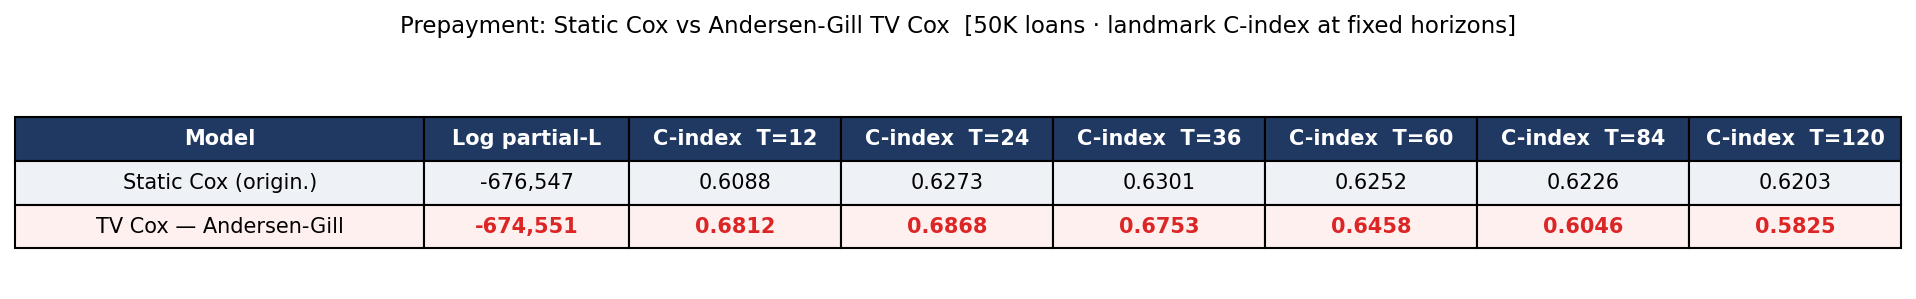
\includegraphics[width=\linewidth]{processed/Eii_model_comparison}
    \caption{Landmark C-index at fixed horizons: Static Cox vs.\ TV Cox Andersen--Gill
      (100K loans, 10K-loan evaluation subsample).
      TV Cox leads at $T=12$--$60$ (peak $+0.072$ at $T=12$, $+0.060$ at $T=24$);
      static Cox overtakes at $T=84$ and $T=120$ as the landmark contamination
      effect overwhelms the TV signal for long-surviving loans.}
\end{figure}

\begin{center}
\small
\begin{tabular}{lrrrrrrrr}
\toprule
\textbf{Model} & \textbf{Log-L} & \textbf{C@T=12} & \textbf{C@T=24}
               & \textbf{C@T=36} & \textbf{C@T=60} & \textbf{C@T=84} & \textbf{C@T=120} \\
\midrule
Static Cox (origination snapshot) & $-676{,}547$ & 0.609 & 0.627 & 0.630 & 0.625 & \textbf{0.623} & \textbf{0.620} \\
\textbf{TV Cox --- Andersen--Gill} & $-674{,}551$ & \textbf{0.681} & \textbf{0.687} & \textbf{0.675} & \textbf{0.646} & 0.605 & 0.583 \\
\midrule
\multicolumn{2}{l}{Part B Macro Cox (1.85M loans, overall C)}
               & \multicolumn{6}{l}{0.6428 (not per-horizon; shown for scale only)} \\
\bottomrule
\end{tabular}
\end{center}

$\Delta$Log-L $= +1{,}996$ confirms that monthly-updated covariates add genuine information
beyond the origination snapshot. TV Cox leads at $T\leq60$; static Cox overtakes
at $T=84$ ($-0.018$) and $T=120$ ($-0.037$), with the crossover near $T\approx70$~months.

% =================================================================
\section{Key Findings and Insights}
% =================================================================

\begin{enumerate}[leftmargin=1.6em,itemsep=3pt]

  \item \textbf{Time-varying covariates add real information.}
        $\Delta$Log-L $= +1{,}996$ (TV vs.\ static, 100K loans) and a $+0.060$ C-index gain
        at $T=24$ confirm that monthly-updated features capture variation invisible to the
        origination snapshot.

  \item \textbf{Short- and medium-horizon gains are large; static Cox overtakes beyond $T\approx70$ months.}
        TV Cox leads by $+0.072$ at $T=12$, $+0.060$ at $T=24$, $+0.045$ at $T=36$,
        and $+0.021$ at $T=60$, then falls below static at $T=84$ ($-0.018$) and
        $T=120$ ($-0.037$). Static Cox is remarkably stable (0.609--0.630 across all horizons),
        while TV Cox degrades monotonically past the 2-year refi peak.

  \item \textbf{Long-horizon degradation is empirically confirmed, not just theoretical.}
        At $T=84$ and $T=120$, surviving loans are a selected group of locked-in,
        high-ELTV borrowers whose current covariate state reflects \emph{why they have not
        prepaid}, not their future risk. The landmark super-model --- conditioning on survival
        to a reference age $s$ then predicting over $(s,\, s+\tau]$ --- is the standard fix.

  \item \textbf{Rate incentive is the key time-varying channel.}
        The current spread $r_{\text{orig}} - r_{\text{market}}(t)$ captures burnout and
        rate cycles invisible to the origination snapshot.
        As the primary rate variable in TV Cox, its coefficient measures the marginal
        refi incentive directly.

  \item \textbf{Unemployment sign flip warns of multicollinearity.}
        High-unemployment periods (2009--2012) coincided with Fed easing and low mortgage rates,
        so unemployment partially proxies for loose monetary policy. Always inspect TV
        coefficients against macroeconomic narratives, not just sign.

  \item \textbf{Synthetic ELTV adds meaningful signal.}
        Equity-unlocking events from HPI appreciation trigger cash-out refis invisible to
        static origination LTV. The negative ELTV coefficient in TV Cox confirms this channel.

\end{enumerate}

\vspace{0.5em}
\textbf{Priority improvements:}
(1) Landmark super-model conditioning on survival to a reference age --- empirically required
    given the $T=84$/$T=120$ degradation observed here.
(2) Vintage-based out-of-time train/test split to produce an unbiased benchmark.
(3) Rolling delinquency indicator --- the largest single missing signal from E(i) ($|\Delta\hat\beta| = 0.543$).

\begin{thebibliography}{9}
\small
\bibitem{ag1982}Andersen, P.\ K.\ and Gill, R.\ D.\ (1982). Cox's regression model for counting processes: a large sample study. \textit{Annals of Statistics} 10:1100--1120.
\bibitem{sadhwani2021}Sadhwani, A., Giesecke, K.\ and Sirignano, J.\ (2021). \textit{J.\ Financial Econometrics} 19:313--368.
\bibitem{cox1972}Cox, D.\ R.\ (1972). Regression models and life tables. \textit{JRSS-B} 34:187--220.
\end{thebibliography}

\end{document}
